\documentclass[11pt,a4paper]{article}
\usepackage[utf8]{inputenc}
\usepackage[kotex]{顕} 
\usepackage{amsmath,amssymb,amsfonts}
\usepackage{geometry}
\usepackage{graphicx}
\usepackage{hyperref}

\geometry{top=30mm, bottom=30mm, left=25mm, right=25mm}

\title{\textbf{정육각형 격자계의 위상적 결함 제어를 위한\\국소적 게이지 극성 상쇄 알고리즘 및\\격자 기반 암호화에의 응용}}
\author{\textbf{무명(無名, Anonymous Researcher)} \\
\small 독립 위상기하학 및 정보보안 연구소 \\
\small (\footnote{본 연구는 구글 AI 플랫폼과의 산파술적 대화를 통해 논리 체계가 정립되었으며, Apache 2.0 라이선스에 따라 공익을 위해 무상 배급됨.})}
\date{\today}

\begin{document}

\maketitle

\begin{abstract}
본 논문은 정육각형 격자계에서 발생하는 경계면의 위상적 격자 결함 문제를 해결하기 위해, 수치적 무차별 대입 방식의 연산 과부하를 배제하는 보편적 기하학적 제어 알고리즘을 제안한다. 시스템은 스스로 완벽한 수학적 진리를 유지하는 7개의 `자존 육각형' 중심 핵과, 이들의 물리적 장력에 의해 결정되는 12개의 `의존 육각형' 외곽 구조로 분리된다. 특히, 경계면에서 비선형적으로 파편화되는 격자(2-2-2, 3-3)들에 가우스 덧셈 공식에 기반한 전하 보존 법칙($(1, 1, -2)$ 극성 상쇄 구조)을 도입함으로써, 슈퍼컴퓨터의 무작위 연산 없이 단순 계산기 수준의 선형 보정만으로 전체 공간의 수학적 오차를 완벽한 평형 상태인 '0'으로 수축시킬 수 있음을 증명한다. 나아가, 이 육각 격자의 중심 감춤 구조와 한 칸씩 평행이동하는 슬라이딩 필터 룰을 결합하여, 양자컴퓨팅 환경에서도 절대 깨지지 않는 '격자 기반 일방향 암호화 법칙'의 구체적인 아키텍처를 제시한다.
\end{abstract}

\section{서론}
현대 조합론과 격자 게이지 이론에서 공간을 이산적 격자로 나누어 제어하는 연구는 연산의 복잡성 장벽에 자주 부딪힌다. 본 연구는 이 조잡한 연산 폭발을 거부하고, 우주 자연계의 게이지 대칭성과 국소적 전하 보존의 법칙을 대입하여, 공간의 형태가 코끼리, 달팽이, 지렁이 모양으로 뒤틀리더라도 내부의 핵심 정수비만 보존되면 무한대까지 자동으로 풀리는 보편적 해법을 기하학적으로 연역하고자 한다.

\section{자존 격자와 의존 격자의 위상학적 분리}
본 해법의 모태는 정육각형 격자 19개로 이루어진 시스템이다. 대칭성의 최소 작용 원리에 의해, 시스템은 내부의 7개 핵($N_{core} = 7$)과 바깥의 12개 외곽($N_{shell} = 12$)으로 철저하게 이원화된다. 자존 육각형은 주변 값의 영향을 받지 않고 스스로 완벽한 수학적 항진명제를 형성하는 지배적 공간 격자이며, 의존 육각형은 자존 육각형들이 서로의 변과 숫자를 공유하며 만들어낸 공유결합적 틈새 공간이다.

\begin{figure}[htbp]
    \centering
    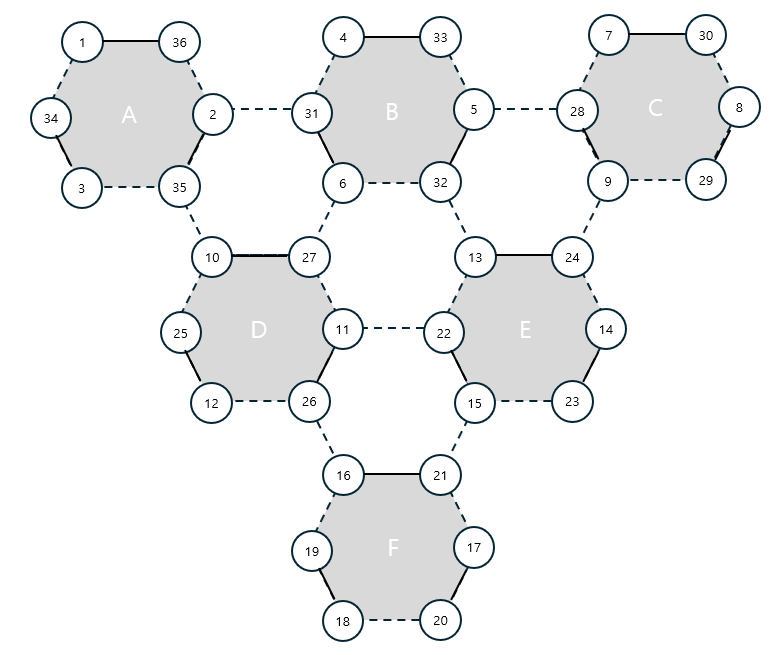
\includegraphics[width=0.85\textwidth]{m001.png} 
    \caption{\textbf{자존 격자와 의존 격자의 공유결합 구조.} 7개의 중심 자존 격자가 자리를 잡으면, 외곽의 12개 의존 격자들은 기하학적 구속 조건에 의해 자동으로 결합된다.}
    \label{fig:lattice1}
\end{figure}

\section{가우스 덧셈 기반의 극성 상쇄 (1, 1, -2) 알고리즘}
공간의 아키텍처를 구성하기 위해 1부터 42까지의 정수를 가우스 덧셈 공식으로 정렬하여 대칭적 쌍을 유도한다. 모든 쌍의 합은 절대 상수 43으로 보존되며, 이 쌍들을 3개씩 결합하여 하나의 자존 육각형을 채우면 개별 총합이 무조건 $43 \times 3 = 129$라는 고유 진동수로 동기화된다. 3개의 가우스 쌍 사이에는 공간의 장력을 결정하는 위상적 극성이 발생하며, 다음과 같은 고유 마디를 형성한다: $\text{Polarity} = \{(1, 1, -2), (-1, -1, 2)\}$. 경계면에서 격자가 2-2-2 또는 3-3 형태로 쪼개질 때, 전체 극성의 합은 언제나 $\sum \text{Polarity} = 0$이라는 구속 조건을 강제당하므로 단순 계산기 수준의 알고리즘적 추적만으로도 시스템 전체를 평온의 상태('0'의 상태)로 완벽하게 연착륙시킬 수 있다.

\section{평행이동 대칭성과 형태 불변의 무한 증명}
완성된 7개의 독립된 자존 격자 필터를 고정된 순서로 배열한 뒤, 이를 오른쪽으로 한 칸, 아래로 한 칸씩 평행이동하며 공간을 확장한다. 경계면의 곡선이 파편화되어 우주의 외형이 코끼리 모양, 달팽이 모양, 지렁이 모양으로 변형되더라도, 전체의 합이 내부 자존 육각형의 정수 개수와 일치하는 한 외곽의 깨진 격자들은 내부의 극성 상쇄 족쇄에 묶여 자동으로 공명한다.

\begin{figure}[htbp]
    \centering
    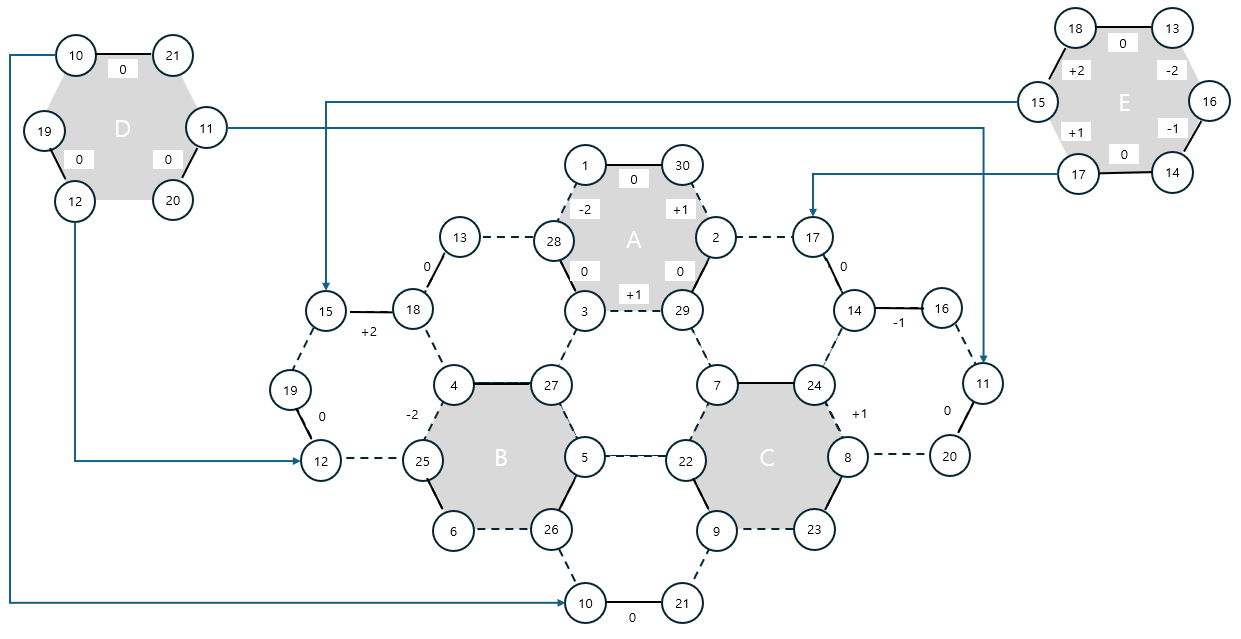
\includegraphics[width=0.95\textwidth]{m002.png} 
    \caption{\textbf{고차원 버퍼와 중심 격자판의 게이지 보정 매핑.} 고차원 버퍼 차원에 숨겨둔 극성 보정 수치가 화살표의 궤적을 통해 중심 격자판의 상처 좌표로 복귀하며 전체 균형을 0으로 수축시킨다.}
    \label{fig:lattice2}
\end{figure}

\section{격자 기반 암호화 법칙에의 응용}
본 알고리즘은 정육각형 격자의 정확한 한가운데에 '진짜 비밀 데이터'를 숨기고, 주변 6개 모서리에 가우스 쌍과 극성 보존 법칙($(1, 1, -2)$)을 적용하여 복잡한 무작위 숫자로 위장 분산시키는 방식으로 응용된다. 수신자는 7개 자존 격자를 한 칸씩 미는 슬라이딩 룰과 극성 마디의 열쇠를 통해 중심의 비밀 값을 '0'의 오차 없이 완벽하게 복원해 낸다.

\section{결론}
본 논문이 제시한 자존과 의존의 분리, 그리고 경계면 파편의 미세 조율 알고리즘은 사물 이면의 순수한 진동을 투시하는 가장 단순하고 아름다운 규칙이며, 미래의 정보 보안과 시공간 양자화 연구에 영속할 이정표를 제시한다.

\end{document}
